% !TEX TS-program = pdflatex
% !TEX encoding = UTF-8 Unicode
% !TEX root = ../2018-03-26-papa-vitres-de-son.tex

%************************************************
\chapter{La Performance}
\label{chp:La Performance}
%************************************************

\begin{quotation}
Since music began to be notated, clearer distinctions between the work and its performance, and between the composer and performer, have emerged, representing multifarious views of the role of the performer.\footnote{Tanja Orning \textit{Pression} (a performance study) Norwegian Academy of MusicMusic Performance Research Copyright © 2012 Royal Northern College of Music Vol. 5}
\end{quotation}

Introduco questo capitolo con una citazione presa da un articolo scritto da Tanja Orning su \textit{Pression} di Helmut Lachenmann. La semplicità con la quale il compositore è riuscito a trasformare il gesto in scrittura è di grande interesse. \begin{wrapfigure}{r}{5cm}
\centering
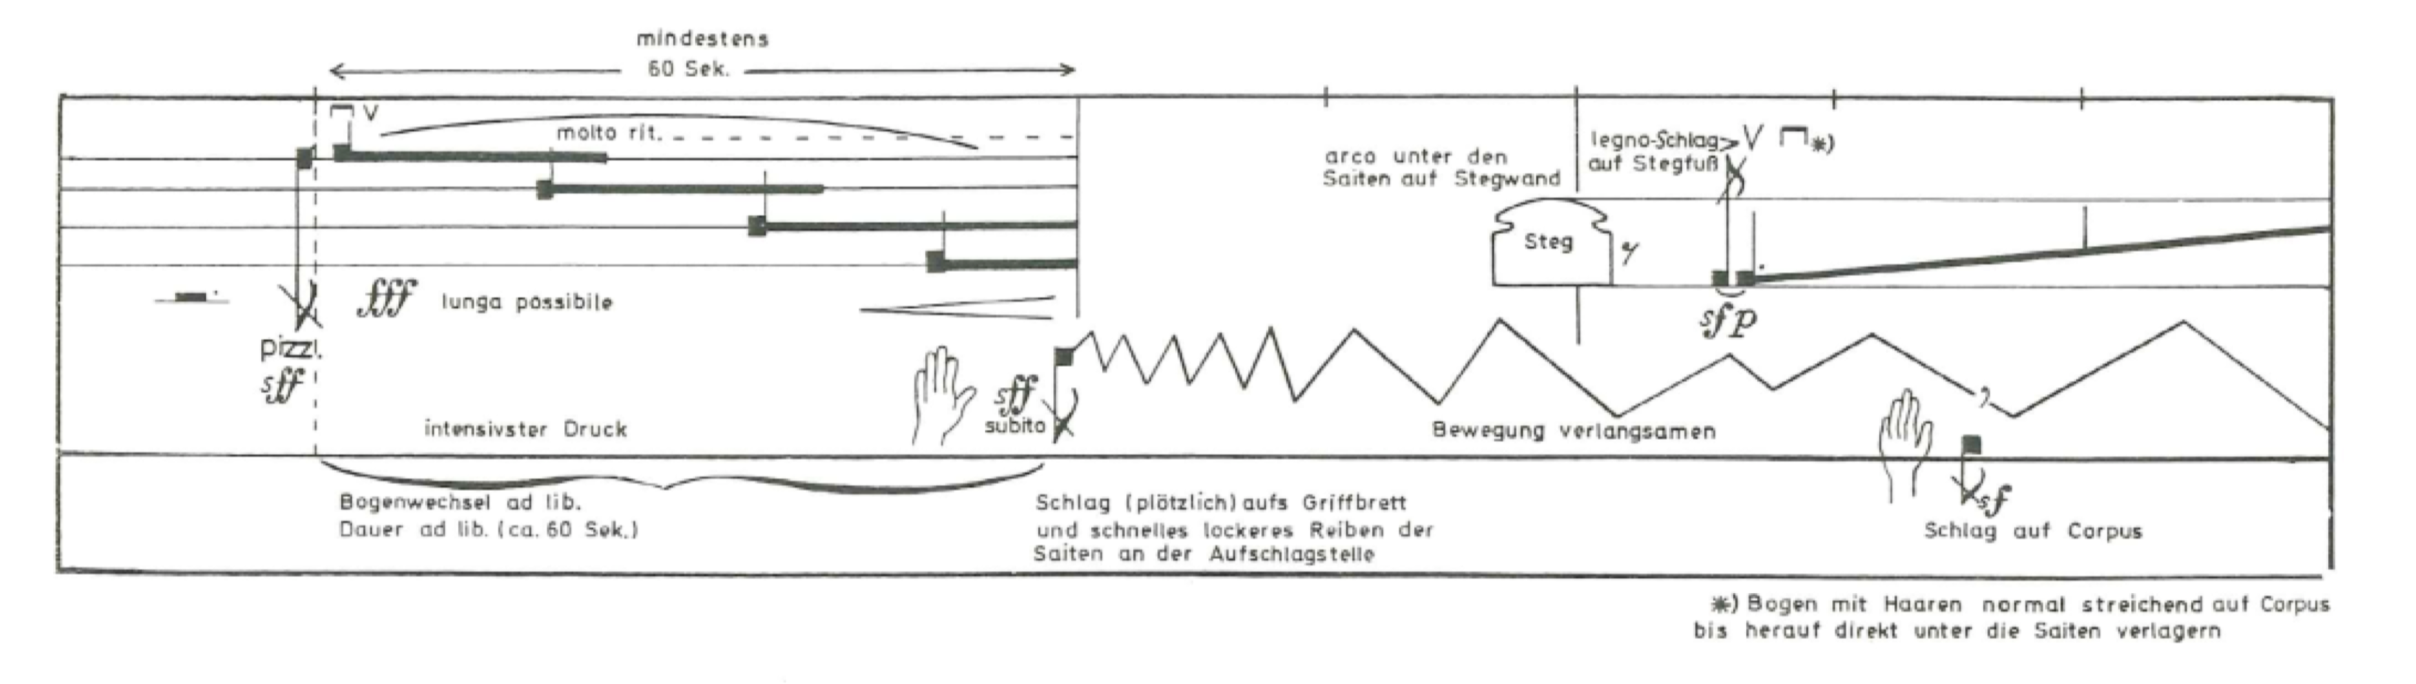
\includegraphics[width=.29\textwidth]{Lachenmann02.jpg}
\caption{particolare partitura \textit{Pression}}
\label{default}
\end{wrapfigure}


\section{Legame tra esecutore/performer e compositore}

Il mio rapporto con gli strumentisti è sempre complicato, dato che, studiando tecniche estese sullo strumento e trovando affascinante capire come si approccia un strumentista al suo strumento, mi ritrovo a modificare continuamente la partiture. La partitura che scrivo durante le prove è quasi un modo per conoscersi, per viversi musicalmente e per vivere lo strumento. Soprattutto in questo caso, dove c'è un primo approccio allo strumento. Matteo Fracassi, studente del dipartimento di percussioni del Santa Cecilia, si è prestato a questo esperimento e ha deciso di intraprendere questo percorso conoscitivo dello strumento addentrandosi nelle maglie della mia scrittura.

 Le difficoltà che intercorrono nel rapporto musicale con il performer sono legate, a mio parere, al simbolo e alla consequenzialità temporale della notazione. Ovvero, se la partitura, nella semiografia e nella scansione temporale, non è puntuale, si possono creare delle incongruenze tra la parte scritta e ciò che si va a suonare. Mi riferisco in particolare al numero di gesti da eseguire sulle molle o sulle placche e alla mancanza di una notazione standard che può far perdere la consequenzialità o la sovrapposizione delle figure ritmiche. Sicuramente, la notazione metronomica e l'utilizzo di accenti facilita la performance, così da dare risalto alle micro-forme interne e alla struttura del pezzo.

\begin{quotation}
I TEMI \\ Non si tratta di opprimere il pubblico con preoccupazioni cosmiche trascendenti. Che possano esservi chiavi profonde del pensiero e dell'azione in base alle quali leggere tutto lo spettacolo[...]. Tuttavia è necessario che queste chiavi esistano; e la cosa riguarda noi\footnote{Antonin Artaud, \textit{Il teatro e il suo doppio}}.
\end{quotation}

Nel lavoro intercorso con il performer, studente del dipartimento di Percussioni del Conservatorio Santa Cecilia, ho riscontrato delle difficoltà nel far recepire il contenuto timbrico e dinamico dei gesti. Essendo un primo approccio, ogni simbolo andava sia spiegato tramite una legenda, sia riproposto in esecuzione da me. Ad esempio, le dinamiche hanno una vita propria. Essendo uno strumento di nuova fattura e amplificato per andare a pescare determinate caratteristiche timbriche, ogni pianissimo parte da una soglia molto bassa di decibel.

Inoltre, Il legame tra gesto e figura è strettamente correlato, dato che, l'approccio ad uno strumento nuovo ha bisogno di una coscienza della correlazione tra il gesto scritto e il risultato sonoro. Ogni gesto avrà bisogno di un riscontro sonoro adeguato per evitare che l'ammaliante timbrica di Sp.I.R.E. porti ad rapportarcisi in modo più improvvisativo che di studio. In pratica, ogni gesto rappresentato in partitura sarà la risultante sonora di un determinato timbro o di una determinata ricerca di armoniche possibili sullo strumento.

Il performer tende quindi a sdoppiarsi tra la figura di esecutore, ma con una capacità performativa estesa alla conformazione dello strumento. Una figura complessa che deve avere la capacità di seguire una struttura compositiva che cercherà di essere la più salda possibile e oltremodo precisa. Questo è la parte da esecutore. E, allo stesso modo, riuscire a districarsi nella lettura di una scrittura "quasi" libera. Per quasi, si intende la libertà minima a livello temporale di prendersi le giuste pause, ma allo stesso tempo riuscire a legare i vari fraseggi che si incastrano, si restringono e si dilatano nel tempo (durata delle frasi) e nello spazio (estensione dello strumento).
